%--------------------------------------------%
% Template Beamer para Apresentações da UFRN %
% by alcemygvseverino@gmail.com              %
% Baseado em MIT Beamer Template			 %
% versao 1.1								 %
% Atualizado em 14/05/2016					 %
%--------------------------------------------%
\documentclass[handout,t]{beamer}
% Para alterar a linguagem do documento
\usepackage[portuges]{babel}
% Para aceitar caracteres especias deretamente do teclado
\usepackage[utf8]{inputenc}
% Para seguir as normas da ABNT de citacao e referencias
\usepackage[alf]{abntex2cite}
% Para incluir figuras
\usepackage{graphicx}
% Para melhor ajuste da posisao das figuras
\usepackage{float}
% Para ajustar as dimensoes do layout da pagina
\usepackage{geometry}
% Para formatar estrutura e informacoes de formulas matematicas
\usepackage{amsmath}
% Para incluir simbolos especiais em formulas matematicas
\usepackage{amssymb}
% Para incluir links nas referencias
\usepackage{url}
% Para incluir paginas de documentos .pdf externos
\usepackage{pgfpages}
% Para ajustar o estilo dos contadores
\usepackage{enumerate}
% Para modificar a cor do texto
\usepackage{color}
% Para incluir condicoes
\usepackage{ifthen}
% Para colocar legendas em algo que nao e float
\usepackage{capt-of}
% Para definir o tema do slide
\usetheme{Berlin}
% Para difinir cores e background
\usecolortheme{ufrn}
% Para numerar as figuras
\setbeamertemplate{caption}[numbered]

% Título
\title[DIM0320]{DIM0320 - Algoritmo e Programação de Computadores}
% Data
\date{\today}
% Autores
\author[M.Musicante]{
	Martin A. Musicante\\%\inst{1}\\
	\vspace{0.25cm}
	\textsl{\small Baseado nas notas de aula de Info 111: Programmation Impérative, Nicolas M. Thiéry, Faculté des Sciences d’Orsay, França}}
% Instituto
\institute[INSTITUTO]{
%	\inst{1}%
	\url{mam@dimap.ufrn.br}\\
	\vspace{0.25cm}
%	\inst{2}%
	Departamento de Informática e Matemática Aplicada}
% Logo do canto inferior direito
\pgfdeclareimage[height=0.7cm]{logo_UFRN}{figuras/logo_UFRN}
\logo{
	\vspace*{-0.25cm}
	\pgfuseimage{logo_UFRN}
	\hspace*{-0.05cm}}


\begin{document}
% Sumário
\frame{\titlepage}
% \section[]{}
% \begin{frame}{Sumário}
% 	\tableofcontents
% \end{frame}

%\section{Introdução}

\begin{frame}{Na última aula: Algoritmos e Programas}
\begin{itemize}
    \item \textbf{Algoritmo:} Descrição de passos para obter um resultado a partir de dados. 
    \\ \qquad (Descrição pode ser pouco rigorosa ou mais abstrata.)
    \item \textbf{Programa:} Implementação de um algoritmo.
    \\ \qquad (Descrição precisa, concreta a ser executada por 
    \\ \qquad \ um computador.)
    \item \textbf{Exemplos:}
    \begin{itemize}
        \item https://youtu.be/RoIY\_vEYglo \item \textit{Hello World} em C: 
        
        \qquad\qquad\qquad\qquad
        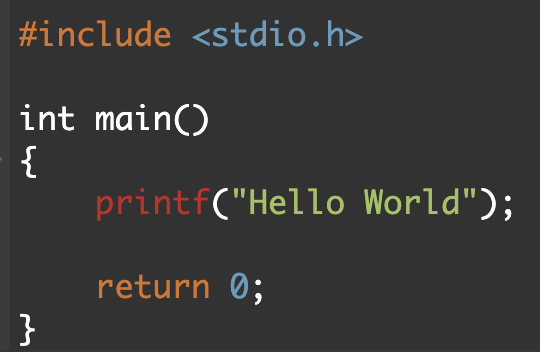
\includegraphics[scale=0.4]{figuras/helloworld.png}
    \end{itemize}
\end{itemize}
\end{frame}

\begin{frame}{Um programa em C}
\begin{itemize}
    \item https://youtu.be/U5U4rVlNIT0 (Prof. Rafael Bezerra).
    \item https://onlinegdb.com/GKHk-I-0A (Hello World):
\begin{center}
    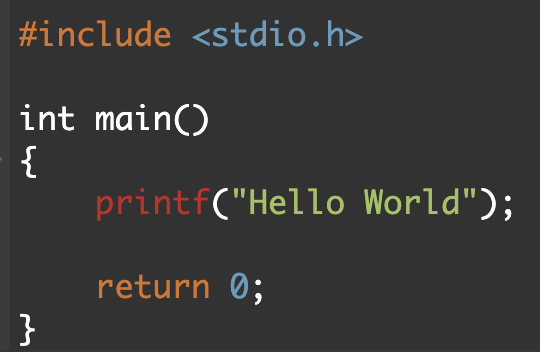
\includegraphics[scale=0.8]{figuras/helloworld.png}
\end{center}
\end{itemize}

O que indica cada linha do programa acima?
\end{frame}

\begin{frame}{Programas e processamento de dados}

\begin{itemize}
    \item Programas servem para processar dados.
    \item Esses dados precisam ser:
    \begin{itemize}
        \item Representados;
        \item Lidos;
        \item Manipulados;
        \item Impressos / gravados para uso posterior.
    \end{itemize}
    \item Representação de dados: Memória do computador.
    \item No texto do programa:
    \begin{itemize}
        \item Constantes / literais;
        \item Variáveis.
    \end{itemize}
\end{itemize}    
\end{frame}

\begin{frame}{Literais, Variáveis, Expressões}
\begin{itemize}
    \item Dentro do programa podem aparecer:
    \begin{itemize}
        \item Valores literais\\
        \qquad- Inteiros: 0, 1023, -434, \dots\\
        \qquad- Reais (ponto flutuante): 3.1415, -345.99, 23344.33, \dots\\
        \qquad- Caracteres: 'a', '2', '@', \dots \\
        \qquad- Strings: "DIMAp", "Jacaré", \dots
        \item Variáveis (identificadores)\\
        \qquad- x23, pi, Distancia, \dots
        \item Expressões podem ser formadas usando literais e identificadores.
    \end{itemize}
\end{itemize}
\end{frame}

\begin{frame}{Expresões}
\begin{itemize}
    \item Expressões são trechos de texto que, quando avaliados, resultam em um valor (resultado da expressão).\\[3mm]
    
    \textbf{Exemplo:} 
    \text{22 - ( -3 + 7 ) + (8 * 5) + (24 / 3)} \\[2mm]
    \qquad resulta em \text{66}
    
    \item Parênteses podem ser aninhados\\[2mm]
    \textbf{Exemplo:} ( 3 * ( 4 + 1) * (3 - (2 + (5 - 7))))
    
    \item Precedência e associatividade dos operadores.\\[2mm]
    \textbf{Exemplo:} 3 * 5 + 2 * 3 + 10 /5\\[2mm]
    \qquad equivale a ((3 * 5) + (2 * 3)) + (10 / 5)
    \item Estas expressões são  \textbf{Expressões aritméticas}.
\end{itemize}
\end{frame}
\end{document}

% Introducao
%\section{Introdução}
\begin{frame}{Introdução}
	A Introdução vai aqui
\end{frame}

% Metodologia
\section{Metodologia}
\begin{frame}{Metodologia}
	Metodologia aqui.
\end{frame}

% Resultados
\section{Resultados}
\begin{frame}{Resultados}
	Resultados do trabalho  
\end{frame}


% Conclusao
\section{Conclusão}
\begin{frame}{Conclusão}
	Conclusões do trabalho  
\end{frame}

% Referencias
\section{Referencias}
\begin{frame}{Referências}
	Suas referencias bibliográficas aqui, siga o modelo ABNT.
	\bibliography{bib/bibliografia}
\end{frame}

% Agradecimentos
\section{}
\begin{frame}{Agradecimentos}
	Agradeço a todos. 	
\end{frame}

\end{document}